\RequirePackage{fix-cm}
\documentclass[smallextended,natbib]{svjour3}
\smartqed
\journalname{Empirical Software Engineering}

\usepackage{graphicx}
\usepackage{amsmath,amssymb}
\usepackage{mathptmx}
\usepackage{booktabs}
\usepackage{array}
\usepackage{xcolor}
\usepackage{listings}
\usepackage{microtype}
\usepackage[hidelinks,breaklinks]{hyperref}

\definecolor{codebg}{HTML}{F4F5F1}
\lstset{
  basicstyle=\ttfamily\footnotesize,
  backgroundcolor=\color{codebg},
  frame=single, framerule=0pt, framesep=6pt,
  breaklines=true, columns=fullflexible, showstringspaces=false,
  aboveskip=8pt, belowskip=8pt, xleftmargin=4pt, xrightmargin=4pt,
}

\newcommand{\code}[1]{\texttt{\small #1}}
\newcommand{\ci}[2]{{\small[#1,\,#2]}}
\newcommand{\authornote}[1]{\textcolor{red}{\textbf{[#1]}}}
\newcommand{\repourl}{https://github.com/trajanovski77/subagent-corpus}

\emergencystretch=1.5em

\begin{document}

\title{Specifying the Machine Team: An Empirical Study of Subagent Definitions in Agentic
Software Development}
\titlerunning{Specifying the Machine Team}

\author{Stefan Trajanovski \and Marko Petrov \and Ema Pandilova \and Ivan Chorbev \and
Dejan Gjorgjevikj}
\authorrunning{S.\ Trajanovski et al.}

\institute{S.\ Trajanovski \and M.\ Petrov \and E.\ Pandilova \and I.\ Chorbev \and D.\ Gjorgjevikj \at
  Faculty of Computer Science and Engineering, Ss.\ Cyril and Methodius University in Skopje,
  1000 Skopje, North Macedonia\\
  Corresponding authors: S.\ Trajanovski, \email{stefan.trajanovski@students.finki.ukim.mk};
  M.\ Petrov, \email{marko.petrov@finki.ukim.mk}\\
  \email{ema.pandilova@finki.ukim.mk}, \email{ivan.chorbev@finki.ukim.mk},
  \email{dejan.gjorgjevikj@finki.ukim.mk}}

\date{Received: date / Accepted: date}

\maketitle

\begin{abstract}
Agentic coding tools let a developer define \emph{subagents}: named delegates, each
with its own instructions, an explicit tool allowlist, a model and a level of autonomy. A subagent
definition is therefore a specification of a machine teammate, and an agent directory is an
organisational chart for non-human labour, checked into version control. Prior work has counted
these files; none has opened them. We present the first content-level study of these
specifications: 50,011 from 3,008 public repositories, analysed at the repository level to respect
strong within-repository dependence. We ask what developers delegate, how much capability they hand
over, and whether their specifications do what they appear to intend. Defect labels come from the
tool itself, through three executable oracles that need neither model inference nor a credential.
Developers do discriminate by role: agents whose declared job is to inspect are granted
file-writing tools 30.7 percentage points less often than agents whose job is to change things.
But the same inspection agents are handed an unrestricted shell, which returns the withheld
capability; fewer than one in five is genuinely read-only, and no role class falls below 84\% able
to write or execute. We confirm the mechanism by execution: an agent holding a shell but no
file-editing tool modifies a file on request. The tool also silently absorbs malformed
configuration, from removed tool names to specifications shadowed by a duplicate name. We report
two of our own claims that execution refuted, and release the corpus, oracles and a linter.
\keywords{agentic software engineering \and AI teammates \and mining software repositories \and configuration defects \and delegation \and least privilege}
\end{abstract}

\section{Introduction}
\label{sec:intro}

Software teams have begun to write down, in version-controlled files, how work should be divided among
AI agents. In Claude Code and comparable tools a developer can define a \emph{subagent}: a named
delegate with a description governing when it is invoked, an explicit tool allowlist, a model
assignment, a permission mode, a turn budget, and an isolation policy. The parent session delegates a
scoped task; the subagent runs in its own context window and returns only a result.

This artifact is unlike the configuration artifacts software engineering usually studies. It is
written mostly in natural language, yet carries hard, machine-enforced fields. It is selected at run
time by a probabilistic model, yet declares privileges enforced deterministically. And, unlike its
sibling artifact \code{settings.json}, it receives \emph{no validation feedback of any kind}: a
specification with a YAML typo does not fail loudly; it simply never exists.

Three properties make it worth studying. First, it is the earliest large-scale observable record of
how practitioners design a division of labour for non-human workers. The multi-agent literature is
rich in \emph{proposed} role architectures (orchestrator, critic, planner, executor) designed by
researchers and evaluated on benchmarks. Here we observe what practitioners specify, in their own
repositories, for their own systems. Second, it encodes privilege decisions: the \code{tools:} field
is an allowlist, so whether a ``reviewer'' is in fact denied write access is a least-privilege
question with a directly measurable answer. Third, it is silently fragile, so ordinary mistakes
persist and accumulate.

\paragraph{Contributions.}
\begin{enumerate}\itemsep2pt
  \item A corpus of 50{,}011 subagent specifications from 3{,}008 public repositories, parsed to a
        structured schema, over $100\times$ the largest previously published sample, released
        with collection code.
  \item Three \emph{executable oracles} that make the coding tool grade its own specifications with
        no model inference and no credential (Section~\ref{sec:oracles}).
  \item A characterisation of delegation design: team size, capability grants, autonomy and cost
        assignment, reported at the repository level to control for extreme concentration.
  \item The \emph{shell-defeats-restriction} result (Section~\ref{sec:privilege}), established
        observationally and confirmed by execution.
  \item A negative methodological result: two of our own oracle-derived claims did not survive
        direct execution, and we report what that implies for oracle-based measurement
        (Section~\ref{sec:oraclelimits}).
  \item A defect census over five classes, each grounded in quoted documentation or an executed
        observation, and a linter that emits the warnings the tool does not.
\end{enumerate}

\section{Background: the subagent artifact}
\label{sec:background}

A subagent is defined by a Markdown file under \code{.claude/agents/} (project scope) or
\code{\textasciitilde/.claude/agents/} (user scope), with YAML frontmatter and a free-text body that
becomes the subagent's system prompt. Table~\ref{tab:schema} summarises the schema.

\begin{table}[t]
\caption{The subagent frontmatter schema and how each field is enforced.}
\label{tab:schema}
\footnotesize
\begin{tabular}{@{}>{\raggedright\arraybackslash}p{2.4cm}>{\raggedright\arraybackslash}p{3.1cm}>{\raggedright\arraybackslash}p{5.5cm}@{}}
\toprule
\textbf{Field} & \textbf{Meaning} & \textbf{Enforcement} \\
\midrule
\code{name} & delegation identifier & required; absent $\Rightarrow$ file ignored \\
\code{description} & governs \emph{when} the parent delegates & required; absent $\Rightarrow$ file ignored \\
\code{tools} & tool allowlist & \textbf{omitted $\Rightarrow$ inherits full tool pool} \\
\code{disallowedTools} & subtractive filter & applied to the inherited set \\
\code{model} & model tier & unknown value $\Rightarrow$ context-window warning \\
\code{permissionMode} & autonomy level & \textbf{ignored when parent is in auto mode} \\
\code{maxTurns} & turn budget & enforced \\
\code{skills}, \code{mcpServers} & capability attachment & ignored for plugin subagents \\
\code{hooks} & lifecycle callbacks & ignored for plugin subagents; needs workspace trust \\
\code{background}, \code{isolation} & execution policy & \code{background} defaults to \code{false} \\
\code{memory}, \code{color} & session policy; UI colour & \code{color} has no runtime effect \\
\bottomrule
\end{tabular}
\end{table}

Two documented semantics \citep{anthropic2026docs} are load-bearing for our analysis.

\begin{quote}
\textbf{S1 (omission is not restriction).} ``Inherits every tool available to subagents if omitted.''
Omitting \code{tools:} is therefore the \emph{most} permissive choice, not a neutral default.
\end{quote}
\begin{quote}
\textbf{S2 (unresolvable tool lists).} The documentation states that ``if no entry in the list
resolves to a tool, the subagent usually fails to launch.'' We tested this directly and it did
\emph{not} hold on build v2.1.233: an agent declaring \code{tools: MultiEdit, LS, TodoRead}, three
names the current release does not recognise, registered normally and completed a task without
error. We therefore treat unresolvable tool names as a \emph{syntactic} defect, not a functional
failure, and report no launch consequence. This is one of two claims that direct execution
refuted; see Section~\ref{sec:oraclelimits}.
\end{quote}

\section{Related work}
\label{sec:related}

\subsection{Mining agentic configuration}

The artifacts that steer coding agents have become a research object in their own right over the past
two years, and the literature has moved outward from the most visible artifact to the more obscure
ones. Context files were first: \citet{chatlatanagulchai2025readmes} study 2{,}303 context files
across 1{,}925 repositories and find that developers write extensively about tests, implementation
detail and architecture, and hardly at all about security or performance. We return to that result,
because it concerns what developers \emph{say} rather than what they \emph{enforce}.
\citet{jiang2026cursorrules} perform the analogous study for editor rule files, deriving a five-part
taxonomy of project context from 401 repositories. Agent skills have been catalogued at very large
scale by \citet{destefanis2026gitskills} and analysed for security by \citet{liu2026agentskills}, who
report that roughly a quarter of more than 31{,}000 marketplace skills carry a vulnerability. Tool
servers have been studied by \citet{hasan2025mcp}.

Closest to us are \citet{galster2026configuring} and the accompanying dataset of
\citet{galster2026dataset}. They inventory eight configuration mechanisms across 2{,}853
repositories and release 18{,}167 configuration files, and theirs is the only prior work to count
subagents at all: 450 of them, in 131 repositories, reported as a distribution (mean 3.44, median 2,
max 17) with no analysis of content. Their dataset paper explicitly names the analysis we perform as
an intended downstream use of their data. We differ in artifact and in depth rather than merely in
scale: we open the frontmatter, model what each field means to the runtime, and measure whether the
declared privilege is the effective one.

A separate line studies what agents \emph{do} rather than how they are configured.
\citet{li2026aidev} assemble a large corpus of agent-authored pull requests, and
\citet{liu2026diveinto} reconstruct the design space of one agent harness from its source, including
its permission modes. The latter is the only prior description of the permission machinery we
measure against; it describes the mechanism, whereas we measure its use in deployed configurations.

\subsection{Agent policy defects}

\citet{chen2026shellsieve} characterise fragility in command \emph{denylists} mined from public
repositories, using an LLM-driven bypass generator validated by sandbox execution, and report that
between 69.0\% and 98.6\% of the denylists they examine fail to block operations they were written to
prevent. Their scope statement is important for positioning ours: they restrict themselves to seven
file-system operations, exclude network operations, and explicitly exclude allowlists, ask-lists,
sandbox settings, hooks, tool-server configuration and subagent tool grants, noting that
``implementation-level defects in the gating layer itself\ldots fall outside our scope.'' Our study is
the complement on all three axes. We study the \emph{allow} side rather than the deny side; we study
the delegation boundary rather than the shell-command boundary; and our defect classes are precisely
the gating-layer ones they set aside.

\subsection{Least privilege and configuration defects}

Least privilege is a founding principle of protection systems \citep{saltzer1975protection}, and the
empirical tradition of testing whether real software honours it is well established. The Android
permission literature is the closest methodological ancestor: \citet{felt2011android} found that about
a third of applications requested permissions they never used, and \citet{au2012pscout} showed that
the mapping from API to permission had to be \emph{extracted from the platform} because the vendor's
documentation of it was incomplete. That lesson, trust the artifact rather than the manual, is the reason
our defect labels come from executing the tool rather than from reading its documentation, and it is
also, as Section~\ref{sec:oraclelimits} reports, the reason two of our own documentation-derived
claims did not survive.

Our contribution differs from classical over-privilege work in one structural respect. Android
over-privilege is a gap between requested and \emph{used} permissions, measured by static analysis of
the application. Here the gap is between the capability the developer withholds and the capability
that remains reachable through a different grant in the same specification. It is a question about
the internal coherence of a policy, not about whether the policy is exercised.

Our defect classes also sit in the configuration-error tradition. \citet{yin2011empirical} established
that a large share of production incidents originate in configuration rather than code, and that
mistakes concentrate in options whose effect is not locally visible. \citet{rahman2019seven} defined
security smells for infrastructure-as-code and, importantly for us, defended each smell as a rule
with a stated rationale rather than a matter of taste. \citet{xu2015knobs} studied configuration
options that are over-designed or effectively unused. That is the nearest prior analogue to our
\emph{inert} classes, where a directive parses, validates, and then does nothing. We follow that
literature's distinction between provable errors and violations of best practice, and we assign every
class we report to the former by grounding it in an executed observation.

\paragraph{Multi-agent role design.}
A large and fast-growing literature proposes role-specialised agent architectures (planner, critic,
executor, orchestrator) and evaluates them on benchmarks. That work studies roles \emph{designed by
researchers} for systems the researchers also built. To our knowledge no prior study examines roles
\emph{specified by practitioners} for their own repositories, at any scale. This is the gap the
present paper occupies, and it is why our role instrument had to be built and validated rather than
borrowed.

\section{Study design}
\label{sec:design}

\subsection{Research questions and data collection}
\begin{itemize}\itemsep2pt
  \item[\textbf{RQ1}] How large are the agent teams developers define, and how concentrated is the
        population?
  \item[\textbf{RQ2}] How much tool capability is granted, and is it narrowed for narrow roles?
  \item[\textbf{RQ3}] If capability is narrowed, is the narrowing effective?
  \item[\textbf{RQ4}] Which fields do developers actually populate?
  \item[\textbf{RQ5}] What fraction of specifications are defective under the tool's own semantics?
\end{itemize}

\paragraph{Collection.}
\label{sec:collection}
Code search on the hosting platform returns at most 1{,}000 results per query and reports unreliable
totals, a well-documented hazard in repository mining \citep{kalliamvakou2016promises}, so we do
not sample from it directly. We use it only to \emph{discover repositories},
partitioning the query space by file size until each partition is retrievable; this yields a frame of
4{,}979 repositories. Each repository is then expanded with a single Git Trees API call returning its
complete file list, from which we extract every agent definition together with every co-located
configuration artifact. This costs one core-API call per repository rather than one search call per
file, and captures files that code search never surfaces. The consequence worth stating plainly is
that \emph{within} a discovered repository our inventory is exhaustive; code search decides only
\emph{which} repositories we look at.

That second step is where the residual bias lives, and we measure it rather than assert its absence.
For every size band we record the reported total, the number of pages actually retrieved, and whether
the reported total exceeded what the interface will serve. Bands in the latter category contribute a
subset of their repositories. In the query log released with the corpus every one of the 28 bands
is in that category, reporting 220{,}220 matching files in total against the 1{,}000 per band the
interface returns, so the frame is a strict subset of the matching population: a same-day re-query
of the same bands retrieved 12{,}251 repositories, among them $99.4\%$ of the frame. Two further
biases follow from the interface itself: forks and non-default branches are not indexed, and
discovery is file-level, so a repository holding many agent files has more opportunities to surface
than one holding few. The repository sample is therefore size-biased toward large agent teams. This
inflates the team-size distribution in Figure~\ref{fig:teamsize}; it has little effect on the
prevalence figures, which are within-repository proportions. The collection script, the per-band
query log and a provenance manifest are released with the corpus.

\subsection{Corpus definition and unit of analysis}
\label{sec:corpus}

Not every \code{.md} file under \code{.claude/agents/} is a subagent specification. Of 67{,}927 files
collected, a substantial minority have no parseable frontmatter or lack the required fields. One
repository in an early snapshot contributed 7{,}175 files, of which 5{,}087 were \code{README.md},
\code{SKILL.md}, \code{TEST\_RESULTS.md} and similar documents living inside the agents directory.

We therefore adopt the tool's own admission requirement as the inclusion criterion: a
\emph{specification} is a file whose frontmatter declares both \code{name} and \code{description}.
This yields \textbf{50{,}011 specifications in 3{,}008 repositories}, or $73.6\%$ of files under the
agents directory. That more than a quarter of the directory's contents are not specifications at all
is itself a finding about how the convention is used.

\paragraph{Unit of analysis.}
\label{sec:unit}
Specifications are not independent. Figure~\ref{fig:concentration} shows the concentration: the
largest repository holds $4.2\%$ of all specifications and the top ten hold $11.0\%$ between them.
Naive specification-level proportions are dominated by a handful of template and generator
repositories.

All prevalence figures are therefore \textbf{repository-level}: the mean of per-repository
proportions, each repository weighted equally, with a percentile bootstrap over repositories
(10{,}000 resamples) for intervals \citep{efron1993bootstrap}. We report the naive pooled figure
alongside wherever the two differ materially. For the headline capability measure the difference is
$33.4\%$ against a pooled $43.7\%$.

\begin{figure}[t]
\centering
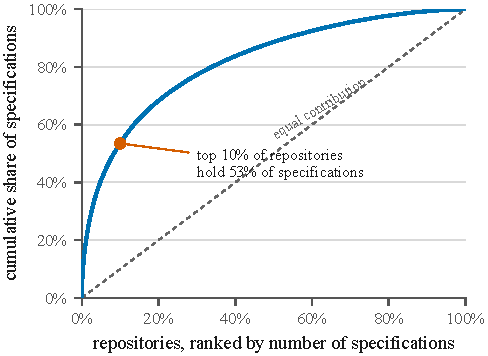
\includegraphics[width=.62\textwidth]{fig1_concentration.pdf}
\caption{Concentration of the corpus. Contribution is uneven, since the top decile of repositories supplies
a disproportionate share of specifications, so specification-level proportions over-represent a
minority of large generator repositories. Every prevalence figure in this paper is therefore
repository-weighted.}
\label{fig:concentration}
\end{figure}

\subsection{Oracles}
\label{sec:oracles}

Configuration-defect studies typically derive labels by reading documentation. We derive them from the
implementation. All three oracles are deterministic, require no model inference and no credential, and
run in under one second per subject.

\paragraph{O1: acceptance oracle.} Invoking the tool with a nonexistent agent name causes it to print
the agents it has successfully loaded. Reconstructing a repository's agents directory and diffing
loaded names against declared names identifies specifications the tool silently discards.

\begin{lstlisting}
$ claude -p "" --agent __probe__ --tools ""
--agent '__probe__' not found. Available agents: architect, code-reviewer, ...
\end{lstlisting}

\paragraph{O2: tool-vocabulary oracle.} Supplying a tool name as a permission rule causes the tool to
emit \emph{matches no known tool} for names it does not recognise. Batched, this yields an
authoritative vocabulary in one invocation. We established 30 valid and 30 invalid names this way;
the invalid set includes the removed legacy names \code{MultiEdit}, \code{LS}, \code{View},
\code{Replace}, \code{NotebookRead}, \code{TodoRead} and \code{SlashCommand}.

\paragraph{O3: settings diagnostic oracle.} For the co-located \code{settings.json} artifact, an
empty-prompt invocation emits per-rule diagnostics on standard error before exiting.

\paragraph{Oracle validation.} We constructed eight specifications exercising known-good and
known-bad forms. O1 accepted the four well-formed cases and silently dropped the four malformed ones
(no frontmatter, missing \code{name}, missing \code{description}, malformed YAML), matching the
documented requirement.

\paragraph{O1 at corpus scale.} We then staged and probed the agent directories of a seeded random
sample of 1{,}591 repositories. The tool listed 23{,}871 of the 23{,}947 specifications our parser
had admitted ($99.7\%$), and specifications in nested sub-directories, which make up $30.5\%$ of the
corpus, loaded as reliably as top-level ones ($99.9\%$ against $99.6\%$). The 76 exceptions are
concentrated in 18 repositories whose agent directories had been reorganised between the corpus
snapshot and the probe, which fetched live files; we cannot separate churn from rejection for them
and do not count them as defects. The admission rule, in other words, is the one the documentation
states, and the corpus inclusion criterion of Section~\ref{sec:corpus} is the tool's own.

\paragraph{What the oracles cannot do.}
\label{sec:oraclelimits}
Oracles are only as good as the construct they observe, and ours are narrower than they first appear.
We state the limits explicitly because two of them falsified claims we had previously drawn.

\begin{enumerate}\itemsep3pt
  \item \textbf{O1 observes registry admission, not launchability.} An agent whose entire
        \code{tools:} list is unresolvable is still listed as available and still runs
        (Section~\ref{sec:background}). O1 therefore cannot support any ``cannot launch'' claim, and
        we make none.
  \item \textbf{O1 is blind to name collisions.} It compares \emph{sets} of names, so two files
        declaring the same \code{name} collapse on both sides. We measure that separately as D6
        (Section~\ref{sec:defects}); it affects 2{,}936 specifications in 144 repositories, and is
        the largest silent-loss mechanism we found.
  \item \textbf{O2 validates the permission namespace, not the frontmatter resolver.} We verified
        that the permission validator suppresses its warning for any candidate containing an
        underscore. \code{my\_bogus\_tool} passes silently while \code{NotARealTool} is flagged, so
        the vocabulary it yields is sound only for underscore-free names. All tool names appearing in
        our corpus that we classify are underscore-free, and MCP tools (which do contain underscores)
        are excluded from the defect count by construction; but the oracle is not a general
        tool-name validator and we do not present it as one.
  \item \textbf{An earlier version of this analysis reported that the tool accepted specifications
        our parser rejected}, and read that as evidence the implementation is more permissive than
        its documentation. It is not: the probe staged \emph{every} file in a repository while the
        declared-name set counted only files our parser could read, so the difference measures our
        own exclusion rule. In the 271 probed repositories where the tool listed names we had not
        registered (1{,}404 names in all), the number of such names never exceeds the number of files
        our parser could not parse. We have withdrawn the claim.
\end{enumerate}

The general lesson is not that executable oracles are unreliable but that they must be validated
against the specific construct in question. Ours were sufficient for registry admission and
vocabulary membership, and insufficient for launchability.

\section{Results}
\label{sec:results}

\subsection{The shape of delegation}

Repositories that define subagents do not define one or two. The mean is $16.6$ specifications per
repository and the median $7$; only $8.3\%$ of repositories define a single agent.
Figure~\ref{fig:teamsize} shows that the distribution is heavy-tailed over three orders of
magnitude. The convention is also very new: Figure~\ref{fig:adoption} dates the repositories in the
corpus and shows that adoption is concentrated almost entirely in the eighteen months preceding
collection ($88.2\%$ of repositories), which is why conventional engineered-project filters are
inapplicable here (Section~\ref{sec:robustness}).

\begin{figure}[t]
\centering
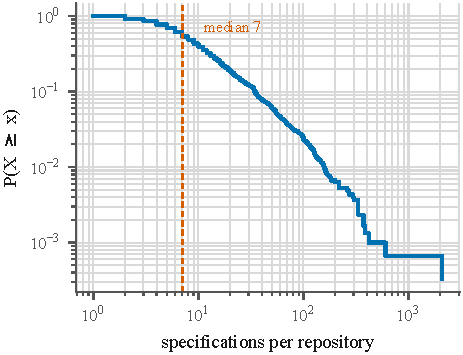
\includegraphics[width=.62\textwidth]{fig2_teamsize.pdf}
\caption{Complementary CDF of team size. A file appearing once per repository would be a preference;
a median of seven with a tail into the thousands is an organisational structure.}
\label{fig:teamsize}
\end{figure}

\begin{figure}[t]
\centering
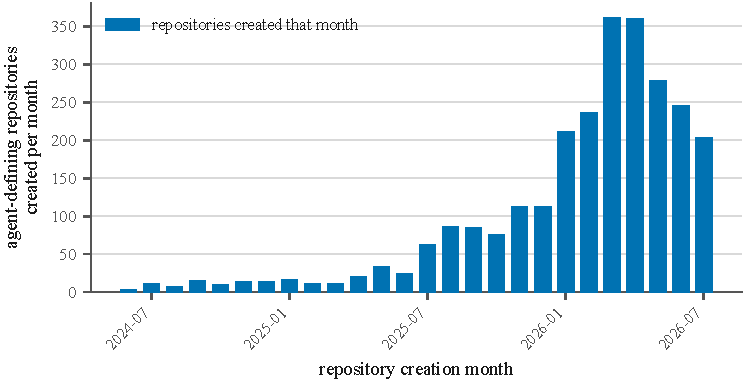
\includegraphics[width=.78\textwidth]{fig9_adoption.pdf}
\caption{When the agent-defining repositories in our corpus were created (the final, partial month is
omitted). The convention is very
young: almost the entire population post-dates the introduction of the subagent format, which is why
standard engineered-project curation (star and age thresholds) would remove most of the corpus and
why we report strata instead (Section~\ref{sec:robustness}).}
\label{fig:adoption}
\end{figure}

\subsection{Capability, role, and the shell}
\label{sec:privilege}

$33.4\%$ \ci{31.8}{35.0} of specifications omit \code{tools:} entirely, which under S1 is the most
permissive choice available. Of those declaring an explicit list, the median grant is six tools.

Because omission \emph{is} maximal privilege, capability must be measured unconditionally. We define
the outcome $W=1$ if a specification can perform the action at all, meaning either it omits \code{tools:}
(and so inherits the full pool) or its explicit list contains a qualifying tool. Conditioning instead
on ``declares an explicit list'', as an earlier version of this analysis did, conditions on a
post-treatment variable that is itself part of the outcome, and systematically understates privilege
for precisely the roles that omit most often.

Whether capability tracks declared role is the substantive question. Because our role labels matter
here, we address measurement error directly. A keyword codebook applied to name and description text
achieved only $\approx\!65\%$ accuracy on a 25-item validation sample. Non-differential
misclassification attenuates between-group contrasts toward zero. That is, a noisy classifier
\emph{manufactures} a ``role does not matter'' result. We therefore restrict the analysis to a
\textbf{high-precision subset}: specifications whose \code{name} field contains exactly one
unambiguous role token ($28.3\%$ of the corpus, $n=14{,}155$). Recall is sacrificed for precision.

On these labels, role clearly predicts privilege. Comparing inspection-oriented roles (reviewer,
security, docs) with change-oriented roles (implementer, debugger), paired within the 924 repositories
that contain both, the difference in the share that can write files is $\mathbf{+30.7}$ percentage
points, 95\%~CI $[27.9, 33.6]$. Developers are practising least privilege, and the effect is large:
reviewers can write files in $49.2\%$ of cases against $96.0\%$ for implementers.

\paragraph{The shell undoes the restriction.}
The restriction does not survive contact with \code{Bash}. Counting shell access as a way to change
things, the same contrast collapses from $30.7$ to $9.2$ points \ci{7.5}{10.9}. More
importantly, the \emph{floor} rises: no role class falls below $84\%$.
Figure~\ref{fig:roleprivilege} shows the two capabilities side by side. For reviewers the gap is the
widest in the corpus: $49.2\%$ can write files, but $85.6\%$ can write files or run a shell. The
absolute level is the finding. Whatever developers intend by withholding \code{Write}, roughly six in
seven reviewer specifications retain a way to change the repository.

\begin{figure}[t]
\centering
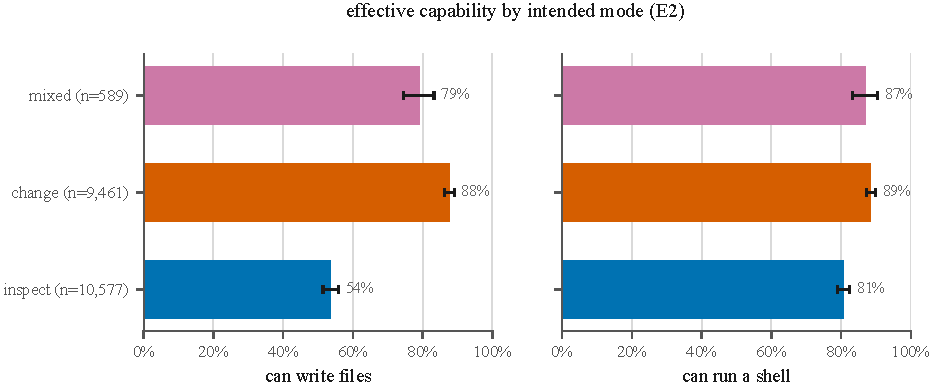
\includegraphics[width=\textwidth]{fig3_role_privilege.pdf}
\caption{Capability by declared role, measured unconditionally (omitting \code{tools:} counts as
holding the capability, since omission inherits the full pool), repository-weighted with 95\%
bootstrap intervals. Developers withhold file-writing tools from inspection roles, then grant those
same roles shell access. The grey connector is the size of the inconsistency; the dashed line marks
the floor below which no role class falls.}
\label{fig:roleprivilege}
\end{figure}

Figure~\ref{fig:heatmap} shows the full picture behind that summary. Read-only inspection tools are
close to universal across every role, as one would expect, with \code{Read} granted by $94$ to $99\%$ of
specifications regardless of role. The two boxed columns carry the argument. \code{Write} varies
sharply and sensibly: $29\%$ for reviewers, $49\%$ for security, $93\%$ for implementers, a spread of
more than sixty points. \code{Bash} barely varies at all: $73\%$, $75\%$ and $89\%$ for the same three
roles, a spread of sixteen. The specification language allows a precise statement of intent,
and developers use it precisely for one capability and bluntly for the capability that subsumes it.

\begin{figure}[t]
\centering
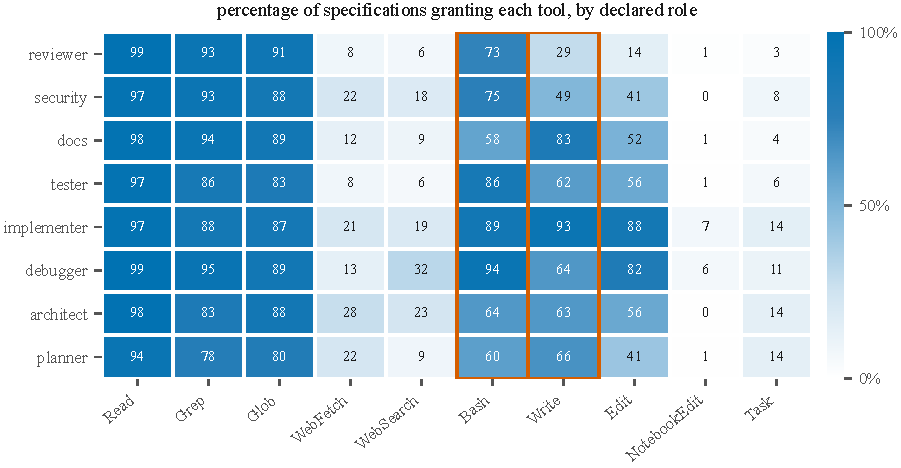
\includegraphics[width=\textwidth]{fig7_heatmap.pdf}
\caption{Tool grants by declared role, restricted to specifications that declare an explicit list.
Cells give the percentage of specifications in that role granting the tool. The boxed columns are the
two that matter: \code{Write} discriminates strongly by role, \code{Bash} barely discriminates at all.}
\label{fig:heatmap}
\end{figure}

Figure~\ref{fig:mechanism} traces the mechanism. Of 3{,}988 inspection-role specifications with an
explicit tool list, $2{,}313$ ($58.0\%$) withhold file-writing tools, so the developer does restrict. But
$1{,}530$ of those $2{,}313$ ($\mathbf{66.1\%}$) grant unrestricted \code{Bash}. Only $783$ ($19.6\%$)
are genuinely read-only. Among inspection specifications granted \code{Bash}, just $2.1\%$ scope it to
particular commands via \code{Bash(...)}; the rest grant the whole shell.

\begin{figure}[t]
\centering
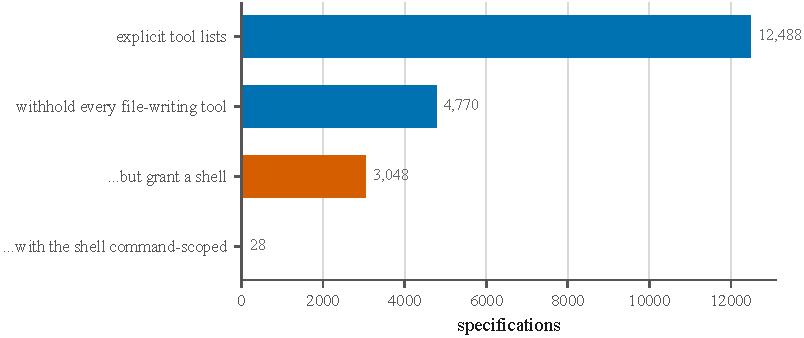
\includegraphics[width=.72\textwidth]{fig4_mechanism.pdf}
\caption{How least privilege is undone. The restriction is real and then void: two-thirds of the
specifications that withhold file-writing tools hand over the shell instead.}
\label{fig:mechanism}
\end{figure}

\paragraph{Confirmation by execution.}
We verified that the restriction is void rather than merely suspicious. We built a specification with
the modal inspection grant of \code{tools: Read, Grep, Glob, Bash}, with no \code{Write} and no
\code{Edit}, and asked the agent to modify a file. Two arms isolate capability from compliance.

\begin{itemize}\itemsep2pt
  \item \textbf{Arm A (neutral system prompt).} The agent modified the file, reaching it through the
        shell with \code{printf 'MODIFIED' | tee target.txt}. The tool blocked the more obvious
        \code{>} redirection, because redirection targets are checked against \code{Edit} rules, but
        \code{tee} passed. \emph{The tool grant did not prevent writing.}
  \item \textbf{Arm B (system prompt states ``you never modify files'').} The agent declined and
        attempted no tool call at all.
\end{itemize}

The operative constraint in Arm B was the prose, not the permission system. A prompt is a
probabilistic guarantee; a tool grant is an enforced one. In this corpus the enforced layer is
routinely left open and the probabilistic layer is asked to carry the weight.

\paragraph{Delegation is adopted ahead of governance.}
\label{sec:cooccurrence}
The pattern is not confined to the \code{tools:} field. Figure~\ref{fig:cooccurrence} places the
agent directory beside the other artifacts in the same repositories. Instruction-shaped artifacts are
common companions: $85.0\%$ of agent-defining repositories also ship a \code{CLAUDE.md}, $60.3\%$ ship
skills, $59.9\%$ run a CI workflow and $43.4\%$ define slash commands. Governance-shaped artifacts
lag: $53.2\%$ ship a \code{settings.json}, $21.1\%$ an \code{.mcp.json}, and $12.6\%$ a local settings
override.
Repositories are adopting delegation faster than they are adopting the machinery that would constrain
it, which is the same ordering we see inside the specification itself.

\begin{figure}[t]
\centering
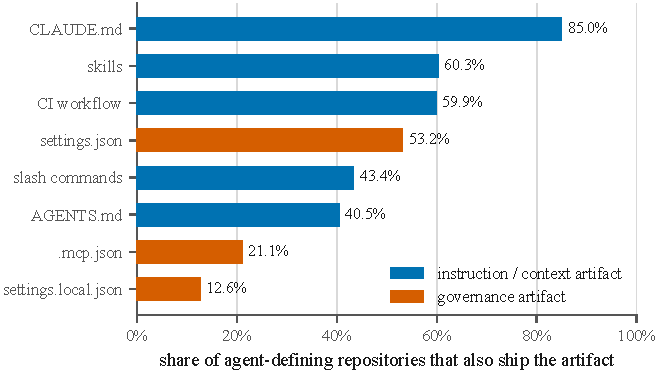
\includegraphics[width=.72\textwidth]{fig8_cooccurrence.pdf}
\caption{What else the agent-defining repositories ship. Instruction and context artifacts (blue) are
widely adopted; governance artifacts (orange) lag behind.}
\label{fig:cooccurrence}
\end{figure}

\subsection{What developers specify, and what is defective}

Developers populate the fields the tool ignores more readily than several it enforces
(Figure~\ref{fig:fields}). A model tier, which is a cost and capability decision, is set by $64.4\%$ of
repositories. A purely cosmetic colour is set by $21.8\%$: thirty times more often than an isolation
policy ($0.7\%$) and ten times more often than \code{disallowedTools} ($2.2\%$). Autonomy is almost
never constrained: \code{permissionMode} appears in $4.1\%$ of repositories, and
even then is inert whenever the parent session runs in auto mode.

\begin{figure}[t]
\centering
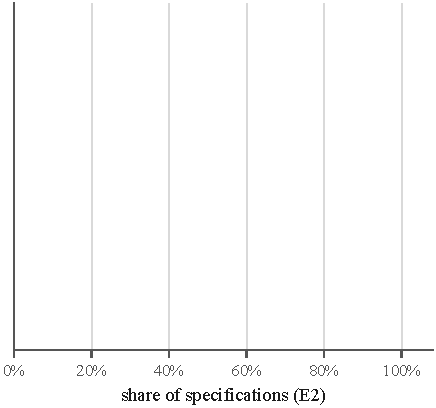
\includegraphics[width=.66\textwidth]{fig5_fields.pdf}
\caption{Share of repositories populating each frontmatter field, repository-weighted with 95\%
bootstrap intervals. The one cosmetic field outranks every capability-constraining field except
\code{model}.}
\label{fig:fields}
\end{figure}

Beyond the schema, $10.7\%$ of repositories use at least one non-schema field (this figure fell once
we added \code{effort} and \code{initialPrompt}, which the documentation does list, to our schema
set). Counted by the repositories that use them, the most common are \code{version} (99 repositories;
3{,}391 specifications), \code{category} (83; 1{,}737), \code{type} (70; 3{,}838),
\code{allowed-tools} (62; 2{,}017), \code{priority} (53; 2{,}671), \code{capabilities} (50; 3{,}229),
\code{author} (44; 2{,}146) and, memorably, \code{emoji} (26; 1{,}996) and \code{vibe} (24; 1{,}984).
None is read by the tool.

\code{allowed-tools} deserves separate mention: it is valid frontmatter for \emph{slash commands}, not
subagents. 2{,}120 specifications use it or a variant (\code{allowedTools}, \code{allowed\_tools}) and
omit the real \code{tools:} field, expressing a restriction the tool never applies and inheriting the
full pool instead. This is $4.2\%$ of specifications but only $1.6\%$ \ci{1.2}{2.0}
repository-weighted, across 73 repositories, and five of those repositories account for 1{,}703 of the
2{,}120 cases: a real defect class, concentrated in a few generator repositories rather than
widespread. We report it as such because the unit of analysis decides the headline.

\paragraph{Defect census.}
\label{sec:defects}
\begin{figure}[t]
\centering
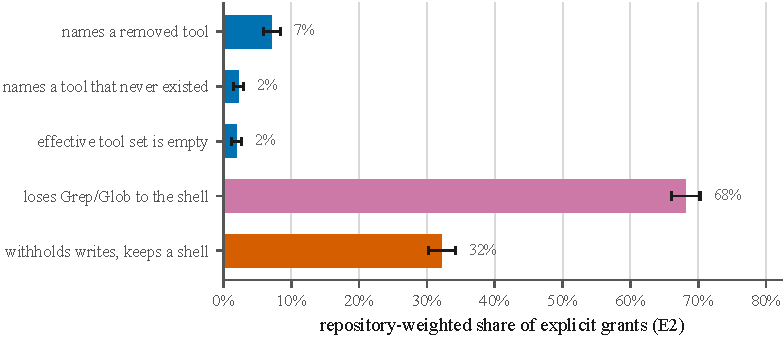
\includegraphics[width=.78\textwidth]{fig6_defects.pdf}
\caption{Defect prevalence, repository-weighted with 95\% bootstrap intervals. Every class is
detected by an executed oracle or by quoted documented semantics.}
\label{fig:defects}
\end{figure}

Figure~\ref{fig:defects} reports the census. $11.6\%$ \ci{10.4}{12.7} of repositories contain a
specification naming at least one tool the current release does not recognise. That class splits
almost evenly, and the split matters for interpretation:

\begin{itemize}\itemsep2pt
  \item \textbf{D2a, artifact--runtime drift} ($6.9\%$ \ci{6.0}{7.8}): names that earlier releases
        genuinely shipped and later removed, such as \code{MultiEdit} (222 repositories; 1{,}860
        occurrences), \code{LS} (148; 1{,}158), \code{TodoRead} (39; 383) and \code{NotebookRead}
        (11; 26). These specifications were plausibly correct when written. They are evidence that
        instruction artifacts rot as their runtime moves, not that their authors were careless.
  \item \textbf{D2b, never-valid names} ($5.5\%$ \ci{4.7}{6.4}): \code{TaskCreate} (56
        repositories), \code{TaskUpdate} (56), \code{TaskList} (49), plus lowercase \code{read},
        \code{search} and \code{todo}. The most striking cases are wholly invented lists such as
        \code{tools: [python,} \code{jupyter,} \code{tensorflow,} \code{pytorch,} \code{huggingface,}
        \code{wandb]} and \code{tools: [Diff Engine,} \code{Impact Analyzer,} \code{Notification Manager,}
        \code{\ldots]}.
\end{itemize}

A specification naming \emph{no} recognised tool at all occurs in $2.0\%$ \ci{1.4}{2.5} of
repositories. We initially expected these agents to be inoperative, since the documentation states
that a fully unresolvable list makes a subagent fail to launch. Direct execution refuted this: such an
agent registers and runs. We therefore report the class as a syntactic defect only.

\textbf{D6, silent shadowing.} $4.8\%$ of repositories declare the same \code{name} on two or more
specifications. Only one can be addressed, so the rest are silently discarded: 2{,}936 specifications
in total. This is the largest silent-loss mechanism in the corpus and, because our acceptance oracle
compares sets of names, it is invisible to O1 and had to be measured separately.

Because the tool emits no diagnostic for any of this, none is discoverable by the developer without
reading the implementation or noticing a silent non-event.

\paragraph{Robustness.}
\label{sec:robustness}
The population skews small: median zero stars, $51.0\%$ with no stars at all, $1{,}510$ of $3{,}008$
carrying a licence, and no forks (code search excludes them). Standard engineered-project curation
\citep{munaiah2017curating} is not directly applicable to a population this young, so
Table~\ref{tab:robust} instead re-estimates the two load-bearing quantities across repository strata.
Both are stable; if anything, omission of \code{tools:} is slightly \emph{more} common in well-starred
repositories.

A second concern is that role cells could be dominated by a few template repositories. Concentration
is modest for most roles and at full corpus size no single repository contributes more than a few
percent of any role. We therefore repeat the headline analysis on a deduplicated sample retaining
\emph{at most one specification per repository per role} (the first in path order), which removes
template domination and reduces the design effect from $6.34$ to $1.64$. On that sample
($n=6{,}871$) the result is essentially unchanged: the file-write contrast is $+28.9$ points
\ci{25.9}{31.9} and the write-or-shell contrast $+8.9$ points \ci{7.0}{10.7}, against $+30.7$ and
$+9.2$ on the full corpus, and no role class falls below $85\%$ able to write or execute. The floor
result is not an artifact of duplicated templates.

\begin{table}[t]
\caption{Robustness of the two load-bearing quantities across repository strata
(repository-weighted, 95\% bootstrap CI). The \code{Bash} column is measured among specifications
that declare an explicit tool list.}
\label{tab:robust}
\small
\begin{tabular}{@{}lrcc@{}}
\toprule
\textbf{Stratum} & \textbf{Repos} & \textbf{Omits \code{tools:}} & \textbf{Grants \code{Bash}} \\
\midrule
All repositories               & 3{,}008 & 33.4\% \ci{32}{35} & 70.8\% \ci{69}{72} \\
$\geq$1 star                   & 1{,}474 & 34.3\% \ci{32}{37} & 71.6\% \ci{70}{74} \\
$\geq$10 stars                 &    665 & 35.4\% \ci{32}{39} & 72.0\% \ci{69}{75} \\
$\geq$50 stars                 &    265 & 38.8\% \ci{33}{44} & 69.4\% \ci{64}{75} \\
Licensed, non-fork             & 1{,}510 & 33.8\% \ci{32}{36} & 71.8\% \ci{70}{74} \\
Excluding repos $\geq$100 specs& 2{,}938 & 32.9\% \ci{31}{35} & 70.7\% \ci{69}{72} \\
\bottomrule
\end{tabular}
\end{table}

\section{Discussion}
\label{sec:discussion}

\subsection{Least privilege is attempted, then defeated}

The most useful thing this corpus says is not that developers are careless. They are not. The gap in
file-writing capability between inspection roles and change roles is large, consistent across every
robustness cut we tried, and cannot plausibly arise by accident: somebody sat down and decided that a
reviewer does not need \code{Write}. That is least privilege, practised deliberately, in a setting
where nothing compels it.

The problem is that the restriction is expressed against the wrong boundary. Withholding \code{Write}
from a reviewer while granting unrestricted \code{Bash} is not a partial restriction; it is no
restriction at all, because the shell is a strict superset of the capability being withheld. Our
execution experiment makes the point concretely: the agent reached the file through
\code{printf | tee} within a few tool calls, having first tried the more obvious shell redirection and
been blocked. That detail is instructive. The tool \emph{does} defend the boundary, since it checks the
target of an output redirection against the file-editing rules, but the defence is enumerative, and
the agent found the case the enumeration missed on its second attempt without being asked to evade
anything.

There is a design lesson here that generalises past this one vendor. A capability list is a sound
abstraction only when its elements are actually independent. \code{Read}, \code{Write} and \code{Edit}
are independent of each other; \code{Bash} is not independent of any of them, because it can
implement all three. Presenting an undifferentiated shell alongside fine-grained file capabilities in
the same allowlist invites exactly the incoherent policy we observe at scale, and no amount of
developer diligence fixes an abstraction that misleads by construction.

\subsection{Prompts, drift, and the absence of feedback}

The second arm of our experiment is quieter but may matter more. When the same tool grant was paired
with a system prompt that said ``you never modify files,'' the agent declined and attempted no tool
call. The constraint that held was the prose, not the permission system.

This is worth stating plainly because it inverts the usual reading of instruction artifacts.
\citet{chatlatanagulchai2025readmes} found that developers rarely write about security in context
files and concluded that guardrails are scarce. Our data suggest something more specific: the
guardrail is often present, but it is present in the wrong layer. Developers write behavioural
constraints in natural language, where compliance is probabilistic and cannot be audited, while
leaving the enforced layer, which is deterministic and auditable, at its most permissive default.
A prompt is a request. A tool grant is a fact. The corpus shows the request doing the work.

A substantial share of the specifications naming unrecognised tools name tools that genuinely
existed and were later removed. These are not authoring errors in any useful sense; they are the
normal consequence of a written artifact outliving the runtime it was written against. The
instruction-artifact literature has so far treated such files as static objects to be characterised.
Our results argue for treating them as objects with a \emph{maintenance} problem: they encode
assumptions about a fast-moving runtime, they are never revalidated, and nothing tells their author
when an assumption expires.

That framing also explains why the sibling artifact behaves better. Permission settings receive
per-rule diagnostics at startup; subagent specifications receive none. The defect rates we report are
close to what one would predict for an artifact with no linter at all, and the cheapest available
intervention is not developer education but a warning message.

\subsection{Implications}

\paragraph{For practitioners.} Omitting \code{tools:} is a privilege decision rather than a default. It
grants everything. A reviewer holding \code{Bash} is not read-only regardless of what its prompt says.
Where a shell is genuinely needed, scope it (\code{Bash(git diff:*)}) or pair it with the sandbox;
otherwise withhold it. Check that every \code{name} in an agent directory is unique, because
duplicates are discarded in silence. The linter released with this paper checks all of this from the
command line and can run in continuous integration.

\paragraph{For tool builders.} Three of our defect classes would be eliminated by diagnostics that
cost nothing to emit: warn when a specification is discarded, when a declared tool does not resolve,
and when a name collides. A fourth, which is the central finding, would be addressed by warning when a
specification withholds file-editing tools but grants an unscoped shell, since that combination is
almost certainly not what its author intended. More structurally, the shell should not sit in the
same undifferentiated allowlist as the capabilities it subsumes.

\paragraph{For researchers.} The executable-oracle method generalises to any configuration artifact
whose runtime can be invoked, and it is cheap: our oracles need no model inference, no credential,
and under a second per subject. But Section~\ref{sec:oraclelimits} is the necessary companion to that
recommendation. An oracle observes one construct, and it is easy to mistake the construct it observes
for the one you care about; we made that mistake twice and caught it only by executing the behaviour
we had inferred.

\section{Threats to validity}
\label{sec:threats}

\paragraph{Construct.} Role labels are derived from the \code{name} field by an automated codebook.
We measured its accuracy ($\approx\!65\%$ on a 25-item sample) and, because misclassification biases
toward the null for our contrast, restricted the headline analysis to a high-precision subset. A
manual coding by two independent annotators reporting Krippendorff's $\alpha$
\citep{krippendorff2004reliability} remains outstanding and is the principal limitation. ``Read-only''
is defined by tool grant, not by observed behaviour; Arm~B of our experiment shows prompts also
constrain behaviour, which we do not measure at scale.

\paragraph{Internal.} All defect classes are relative to a pinned build (v2.1.233); the tool
vocabulary changes between releases, so a specification may have been valid when authored. Dating
defects against the introducing commit is outstanding. The inertness of \code{permissionMode} depends
on the parent session's mode, which is unobservable from the repository, so we report it as
conditional. Our corpus inclusion rule requires parseable frontmatter, which biases toward well-formed
specifications and therefore likely \emph{under}-estimates defect rates.

\paragraph{External.} This is a convenience sample, not a probability sample, and we make no
population estimate. Three specific biases are worth naming. \emph{(i)~Ordered expansion.} Repository
expansion is complete: all 4{,}979 frame repositories were expanded, of which 3{,}008 contain at least
one specification. Table~\ref{tab:robust} shows the two load-bearing quantities are stable across
quality strata.
\emph{(ii)~Size-biased discovery.} Discovery is file-level: a repository with $n$ matching files has
$n$ chances to surface in some partition, so inclusion probability rises with team size and the
team-size distribution in Figure~\ref{fig:teamsize} is biased upward. Prevalence figures, being
within-repository proportions, are far less affected. \emph{(iii)~Truncation.} Each size partition
was retrieved to a fixed page depth, and every partition had more results than that depth, so all
are truncated and the frame under-samples the matching population.
File size correlates with the number of tools granted (Spearman $\rho=0.32$) but not with the
omit/declare binary ($\rho<0.01$), so the headline capability measure is not confounded by this while
tool-count statistics should be read with care.

The population also skews young and small: median zero stars, $51.0\%$ with no stars at all. Standard
engineered-project curation would delete most of the corpus in an ecosystem this new, so we report
strata instead of filtering. Findings concern one vendor's format. The \emph{phenomenon} itself, a
declarative delegation artifact with an enforced privilege field, is not vendor-specific, but the
rates are.

\paragraph{Conclusion validity.} Specifications within a repository are strongly dependent. For the
write/exec outcome the intra-class correlation is $\mathrm{ICC}=0.41$ over 27{,}747 specifications in
1{,}980 repositories, giving a design effect of $6.34$: the effective sample size is $4{,}373$, not
$27{,}747$. Any analysis treating specifications as independent would understate uncertainty roughly
six-fold.
All prevalence figures therefore use the repository as the unit of analysis with percentile bootstrap
intervals over repositories, and the role contrast is paired within the repositories that contain both
groups, which additionally controls for repository-level authoring style. A further dependence remains
unmodelled: $30.9\%$ of specifications are byte-identical to a file appearing in at least one other
repository, so repositories are not fully independent clusters either.

\section{Conclusion}
\label{sec:conclusion}

Developers have begun to write down how work is divided among machines, and we studied that record at
scale for the first time. They build large teams that mirror human software organisations, and they
genuinely practise least privilege when granting file-writing tools, a $30.7$-point gap between
roles that inspect and roles that change. They then hand two-thirds of the restricted agents an
unrestricted shell, which returns the capability they had just withheld; only about one inspection
agent in five is genuinely read-only. Because the tool never objects, one repository in nine also
ships a specification naming a tool the current release does not recognise, one in fifty ships a
tool list that resolves to nothing at all, and one in twenty declares the same agent name twice so
that one copy is never loaded. The org chart is in the repository. The guardrails are drawn against
the wrong boundary.

\section*{Declarations}

\paragraph{Funding}
\authornote{Authors to complete, e.g.\ ``The authors did not receive support from any organisation
for the submitted work.''}

\paragraph{Conflict of interest}
The authors declare that they have no conflict of interest. \authornote{Authors to confirm.}

\paragraph{Ethics approval and consent to participate}
Not applicable. The study analyses publicly available repository content and involved no human
participants.

\paragraph{Consent for publication}
Not applicable.

\paragraph{Data availability}
The corpus (50{,}011 parsed specifications with raw frontmatter values, the per-repository
configuration inventories, repository metadata, and the acceptance-oracle output), the tool
vocabulary established by O2, and the complete analysis output are archived at Zenodo
\authornote{DOI to be minted before submission} and maintained at \url{\repourl}.
All tool behaviour reported here was observed on Claude Code v2.1.233, commit \code{f8d57569aaf3}.

\paragraph{Code availability}
The collection script, the acceptance oracle, the analysis and figure scripts, and the linter are
released in the same archive and at \url{\repourl}. Code is licensed under the MIT licence and the
corpus under CC~BY~4.0.

\paragraph{Author contribution}
\authornote{CRediT statement to be completed by the authors.}

\bibliographystyle{spbasic}
\bibliography{refs}

\end{document}
